% !TEX root = ./Main.tex
\documentclass[11pt,a4paper]{article} 

\usepackage{titlesec}
\usepackage{color}

% PACKAGES FOR LANGUAGE AND FONT
\usepackage[utf8]{inputenc}
%\usepackage[english]{babel}
\usepackage[italian]{babel}
\usepackage[T1]{fontenc} % Font encoding

% PACKAGES FOR IMAGES
\usepackage{graphicx}
\graphicspath{{Images/}}
\usepackage{eso-pic} % For the background picture on the title page
\usepackage{subfig} % Numbered and caption subfigures using \subfloat
\usepackage{caption} % Coloured captions
\usepackage{transparent}


% STANDARD MATH PACKAGES
\usepackage{amsmath}
\usepackage{amsthm}
\usepackage{bm}
\usepackage[overload]{empheq}  % For braced-style systems of equations

% PACKAGES FOR TABLES
\usepackage{tabularx}
\usepackage{longtable} % tables that can span several pages
\usepackage{colortbl}

% PACKAGES FOR ALGORITHMS (PSEUDO-CODE)
\usepackage{algorithm}
\usepackage{algorithmic}

% PACKAGES FOR REFERENCES & BIBLIOGRAPHY
\usepackage[colorlinks=true,linkcolor=black,anchorcolor=black,citecolor=black,filecolor=black,menucolor=black,runcolor=black,urlcolor=black]{hyperref} % Adds clickable links at references
\usepackage{cleveref}
\usepackage[square, numbers, sort&compress]{natbib} % Square brackets, citing references with numbers, citations sorted by appearance in the text and compressed
\bibliographystyle{unsrt} % You may use a different style adapted to your field
%\bibliographystyle{plain}


% PACKAGES FOR THE APPENDIX
\usepackage{appendix}

% PACKAGES FOR ITEMIZE & ENUMERATES 
\usepackage{enumitem}

% OTHER PACKAGES
\usepackage{amsthm,thmtools,xcolor} % Coloured "Theorem"
\usepackage{comment} % Comment part of code
\usepackage{fancyhdr} % Fancy headers and footers
\usepackage{lipsum} % Insert dummy text
\usepackage{tcolorbox} % Create coloured boxes (e.g. the one for the key-words)

\usepackage[european, RPvoltages, siunitx, straightvoltages]{circuitikz}
\usepackage{pgfplots}
\pgfplotsset{width=10cm,compat=1.6}

%-------------------------------------------------------------------------
%	NEW COMMANDS DEFINED
%-------------------------------------------------------------------------
% EXAMPLES OF NEW COMMANDS -> here you see how to define new commands
\newcommand{\bea}{\begin{eqnarray}} % Shortcut for equation arrays
\newcommand{\eea}{\end{eqnarray}}
\newcommand{\e}[1]{\times 10^{#1}}  % Powers of 10 notation
\newcommand{\mathbbm}[1]{\text{\usefont{U}{bbm}{m}{n}#1}} % From mathbbm.sty
\newcommand{\pdev}[2]{\frac{\partial#1}{\partial#2}}
% NB: you can also override some existing commands with the keyword \renewcommand

%----------------------------------------------------------------------------
%	ADD YOUR PACKAGES (be careful of package interaction)
%----------------------------------------------------------------------------


%----------------------------------------------------------------------------
%	ADD YOUR DEFINITIONS AND COMMANDS (be careful of existing commands)
%----------------------------------------------------------------------------


% File di configurazione Configuration_files/config.tex  
% Configuration package
\usepackage[bottom=2.0cm,top=2.0cm,left=2.0cm,right=2.0cm]{geometry}
\raggedbottom 

% --- MODIFICA INTERLINEA ---
\usepackage{setspace}
\onehalfspacing % Usa \setstretch{1.25} se 1.5 ti sembra troppo
% ---------------------------

% Create color RED_SST
\definecolor{RED_SST}{rgb}{0.6,0.1,0.1}

% Custom theorem environments
\declaretheoremstyle[
  headfont=\color{RED_SST}\normalfont\bfseries,
  bodyfont=\color{black}\normalfont\itshape,
]{colored}

\captionsetup[figure]{labelfont={color=RED_SST}} % Set colour of the captions
\captionsetup[table]{labelfont={color=RED_SST}} % Set colour of the captions
\captionsetup[algorithm]{labelfont={color=RED_SST}} % Set colour of the captions

\theoremstyle{colored}
\newtheorem{theorem}{Theorem}[section]
\newtheorem{proposition}{Proposition}[section]

% Enhances the features of the standard "table" and "tabular" environments.
\newcommand\T{\rule{0pt}{2.6ex}}
\newcommand\B{\rule[-1.2ex]{0pt}{0pt}}

% Algorithm description
\newcounter{algsubstate}
\renewcommand{\thealgsubstate}{\alph{algsubstate}}
\newenvironment{algsubstates}{
    \setcounter{algsubstate}{0}%
    \renewcommand{\STATE}{%
    \stepcounter{algsubstate}%
    \Statex {\small\thealgsubstate:}\space}
    }{}
    
% Custom theorem environment
\newcolumntype{L}[1]{>{\raggedright\let\newline\\\arraybackslash\hspace{0pt}}m{#1}}
\newcolumntype{C}[1]{>{\centering\let\newline\\\arraybackslash\hspace{0pt}}m{#1}}
\newcolumntype{R}[1]{>{\raggedleft\let\newline\\\arraybackslash\hspace{0pt}}m{#1}}

% Custom itemize environment
\setlist[itemize,1]{label=$\bullet$}
\setlist[itemize,2]{label=$\circ$}
\setlist[itemize,3]{label=$-$}
\setlist{nosep}

% Create command for background pic
\newcommand\BackgroundPic{% Adding background picture
	\put(240,370){
	    \parbox[b][\paperheight]{\paperwidth}{%
	    \vfill
		\centering
		\transparent{0.1}
		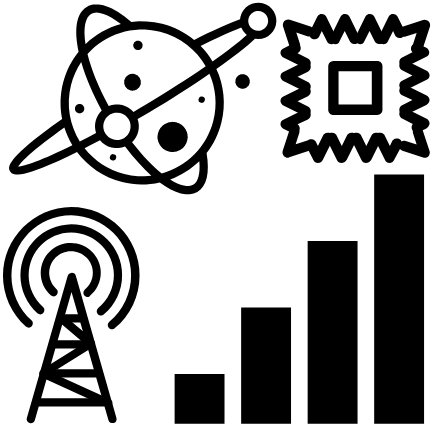
\includegraphics[width=0.14\paperwidth]{Images/logo_GB.png}%
		\vfill}
		}
}

% Set indentation
\setlength\parindent{0pt}

% Custom title commands
\titleformat{\section}
{\color{RED_SST}\normalfont\Large\bfseries}
{\color{RED_SST}\thesection.}{1em}{}
\titlespacing*{\section}
{0pt}{3.3ex}{3.3ex}

\titleformat{\subsection}
{\color{RED_SST}\normalfont\large\bfseries}
{\color{RED_SST}\thesubsection.}{1em}{}
\titlespacing*{\subsection}
{0pt}{3.3ex}{3.3ex}

% Custom headers and footers
\pagestyle{fancy}
\fancyhf{}
      
\fancyfoot{}
\fancyfoot[C]{\thepage} % page
\renewcommand{\headrulewidth}{0mm} % headrule width
\renewcommand{\footrulewidth}{0mm} % footrule width

\makeatletter
\patchcmd{\headrule}{\hrule}{\color{black}\hrule}{}{} % headrule
\patchcmd{\footrule}{\hrule}{\color{black}\hrule}{}{} % footrule
\makeatother

 
\renewcommand{\title}{Modulazione AM e Demodulazione di un segnale}
\renewcommand{\author}{Martina Coros}
\newcommand{\secondAuthor}{Samuele Verna}
\newcommand{\course}{Analisi ed Elaborazione dei Segnali}
\newcommand{\firstadvisor}{Prof. Fortunato SANTUCCI}
\newcommand{\secondadvisor}{Prof. Piergiuseppe DI MARCO}
\newcommand{\firstcoadvisor}{Dr. Graziano BATTISTI} % insert if any otherwise comment
\newcommand{\secondcoadvisor}{Dr. Graziano BATTISTI} % insert if any otherwise comment
\newcommand{\ID}{Matr. 111111}
\newcommand{\secondID}{Matr. 309996}
\newcommand{\YEAR}{2025-2026}

\renewcommand{\abstract}{In questo esperienza di laboratorio si è studiata la modulazione in ampiezza (AM) e la demodulazione di un segnale, processo fondamentale per la trasmissione dell'informazione in un contesto reale. Nel corso del laboratorio si sono realizzate tutte le fasi del processo, dalla generazione del segnale modulante alla modulazione del segnale portante, fino alla demodulazione del segnale ricevuto tramite l'utilizzo di un circuito e di un filtro. Durante l'esperimento sono state analizzate le caratteristiche dei segnali ottenuti tramite l'oscilloscopio. I risultati ottenuti hanno permesso di comprendere meglio i principi fondamentali del processo, nonché le applicazioni pratiche di queste tecniche nella trasmissione dei segnali.
}

\newcommand{\keywords}{Modulazione AM, Demodulazione, FFT, Filtro Passa-Banda, Teoria dei Segnali}

%-------------------------------------------------------------------------
%	BEGIN OF YOUR DOCUMENT
%-------------------------------------------------------------------------
\begin{document}

%-----------------------------------------------------------------------------
% TITLE PAGE
%-----------------------------------------------------------------------------
% DO NOT REMOVE SPACES BETWEEN LINES!

%\AddToShipoutPicture*{\BackgroundPic}
\begin{center}
    
\includegraphics[width=0.7\textwidth]{Images/logo_doppio.png}
\end{center}

\vspace{10mm}
\begin{center}
    \Large{\textbf{\color{RED_SST}{\title}}}\\
\end{center}

\vspace{4mm}
\begin{center}
    \fontsize{0.3cm}{0.5cm}\selectfont \bfseries \textsc{\color{RED_SST} Relazione attività Laboratorio SST  \\ \course}\\
\end{center}

\vspace{4mm}
\begin{center}
    \large{\textbf{\author, \ID}}

    \large{\textbf{\secondAuthor, \secondID}}
\end{center}

\small \normalfont

\vspace{11pt}

\centerline{\rule{1.0\textwidth}{0.4pt}}

\begin{center}
    \begin{minipage}[t]{.28\textwidth}
        \begin{minipage}{.90\textwidth}
            \noindent
            \scriptsize{\textbf{Advisors:}} \\
                \firstadvisor \\
                \secondadvisor \\
            \\
            \textbf{Co-advisor:} \\ 
                \firstcoadvisor \\ 
                %\secondcoadvisor \\ 
            \textbf{Academic year:} \\
                \YEAR \\
            \\
        \end{minipage}
    \end{minipage}
    \begin{minipage}{.70\textwidth}
        \noindent \textbf{\color{RED_SST} Sommario:} {\abstract}
    \end{minipage}
\end{center}

\vspace{15pt}

\begin{tcolorbox}[arc=0pt, boxrule=0pt, colback=RED_SST!60, width=\textwidth, colupper=white]
    \textbf{Key-words:} \keywords
\end{tcolorbox}

\vspace{12pt}

%%%%%%%%%%%%%%%%%%%%%%%%
%%      MAIN TEXT     %%
%%%%%%%%%%%%%%%%%%%%%%%%

%-----------------------------------------------------------------------------
% INDICE
%-----------------------------------------------------------------------------

\newpage
\tableofcontents
\newpage

%-----------------------------------------------------------------------------
% CAPITOLI
%-----------------------------------------------------------------------------
\section{Introduzione e Obiettivi}
\label{sec:Introduzione}
\thispagestyle{plain}
L'obiettivo di questo progetto è quello di realizzare un sistema di elaborazione dei segnali
\section{Cenni Teorici}
\label{sec:Teoria}
\thispagestyle{plain}
In questa sezione vengono riportati alcuni cenni teorici sui concetti fondamentali dell'analisi dei segnali, che sono stati utilizzati durante lo sviluppo del progetto. Verranno trattati argomenti come la rappresentazione dei segnali, la trasformata di Fourier, il campionamento e la ricostruzione dei segnali, nonché alcune tecniche di filtraggio e analisi spettrale. Questi concetti forniscono le basi teoriche necessarie per comprendere le operazioni svolte sui segnali durante l'esperimento e per interpretare i risultati ottenuti.

\subsection{Trasformata di Fourier}
Per poter analizzare ed elaborare i segnali, bisogna spesso ricorrere ad una loro rappresentazione alternativa, che permetta di evidenziare alcune caratteristiche che non sono immediatamente visibili nella rappresentazione temporale. La trasformata di Fourier è uno strumento matematico che consente di rappresentare un segnale come somma di sinusoidi di frequenze diverse, fornendo così una rappresentazione in frequenza del segnale stesso. 

\subsubsection{DFS: Discrete Fourier Series}
La Trasformata di Fourier è definita per segnali continui, ma nella pratica si lavora con segnali discreti, campionati ad intervalli regolari. La Discrete Fourier Seriers (DFS) è una verisione discreta della trasformata Serie di Fourier, che permette di rappresentare una sequenza di campioni periodica come somma finita di armoniche complesse. La DFS è definita come segue:

\begin{equation}
    \label{sec:DFS}
    X[k] = \sum_{n=0}^{N-1} x[n] e^{-j \frac{2\pi}{N} kn}
\end{equation}
dove $x[n]$ è la sequenza di campioni del segnale, $N$ è il numero totale di campioni (per gli oscilloscopi generalmente 1024) e $X[k]$ è la componente in frequenza corrispondente alla frequenza $k$.

\subsubsection{DFT: Discrete Fourier Transform}
La Discrete Fourier Transform (DFT) è una generalizzazione della DFS che permette di rappresentare una sequenza di campioni non necessariamente periodica. La DFT è definita come segue:

\begin{equation}
    \label{sec:DFT}
    X[k] = \begin{cases}
    \sum_{n=0}^{N-1} x[n] e^{-j \frac{2\pi}{N} kn} & \text{se } 0 \leq k < N\\
    0 & \text{altrimenti}
    \end{cases}
\end{equation}
dove $x[n]$ è la sequenza di campioni del segnale, $N$ è il numero totale di campioni (per gli oscilloscopi generalmente 1024) e $X[k]$ è la componente in frequenza corrispondente alla frequenza $k$.

\subsubsection{FFT: Fast Fourier Transform}
Dall'equazione \ref{sec:DFT}, si può notare che il calcolo della DFT per una singola frequenza $k$ richiede sommare $N$ prodotti, e quindi il calcolo della DFT per tutte le frequenze ha una complessità di \textbf{$O(N^2)$} operazioni. Considerando che negli oscilloscopi si lavora generalmente con $N=1024$ campioni, il calcolo diretto della DFT sarebbe particolarmente oneroso. 

Per superare questo limite prestazionale, si ricorre alla \textbf{Fast Fourier Transform (FFT)}. Non si tratta di una nuova definizione matematica rispetto alla DFT, ma di una classe di algoritmi altamente ottimizzati per il suo calcolo. 

L'algoritmo più noto (introdotto da Cooley e Tukey) sfrutta le proprietà di simmetria e periodicità dell'esponenziale complesso e utilizza un approccio di tipo \textit{divide et impera} (divide and conquer). Se il numero di campioni $N$ è una potenza di 2 (come è tipico nelle architetture digitali e negli oscilloscopi), l'algoritmo suddivide iterativamente il calcolo della trasformata di lunghezza $N$ in trasformate di lunghezza decrescente (pari e dispari).

Questa scomposizione abbatte drasticamente il numero di moltiplicazioni e addizioni necessarie, riducendo la complessità computazionale da $O(N^2)$ a $O(N \log_2 N)$. 

Per comprendere l'impatto pratico di questa ottimizzazione, riprendiamo l'esempio dell'oscilloscopio che elabora $N = 1024$ campioni:
\begin{itemize}
    \item \textbf{Con la DFT diretta:} sarebbero necessarie circa 1.048.576 operazioni ($1024^2$).
    \item \textbf{Con l'algoritmo FFT:} sono sufficienti solamente 10.240 operazioni ($1024 \times 10$).
\end{itemize}

Questo abbattimento del carico computazionale (un fattore di riduzione di circa 100 volte in questo caso specifico) è l'elemento chiave che permette alla strumentazione di laboratorio e ai moderni calcolatori di eseguire l'analisi spettrale e la visualizzazione dei segnali in tempo reale.

\subsubsection{Considerazioni pratiche sull'uso della FFT all'oscilloscopio}

Nell'utilizzo dell'oscilloscopio per la FFT, bisogna bilanciare due aspetti cruciali: la risoluzione in frequenza e il limite di fondo scala. Dato che lo strumento elabora un numero fisso di campioni (generalmente $N = 1024$), modificare la scala dei tempi altera direttamente la frequenza di campionamento ($f_c$). 

La durata complessiva della finestra temporale è definita come:
$$T = \frac{N}{f_c}$$

Se allarghiamo la finestra temporale per includere più oscillazioni del segnale (aumentando $T$), lo strumento è costretto a campionare più lentamente (diminuendo $f_c$). Questo comporta due conseguenze pratiche:

\begin{itemize}
    \item \textbf{Aumento della risoluzione in frequenza:} La distanza $\Delta f$ tra i campioni nello spettro è data da $\Delta f = \frac{1}{T} = \frac{f_c}{N}$. Aumentando il tempo di osservazione $T$, il passo $\Delta f$ si riduce, permettendo di distinguere con maggiore precisione le singole componenti in frequenza (es. le delta di Dirac).
    
    \item \textbf{Riduzione del fondo scala:} Per il teorema del campionamento di Nyquist, la frequenza massima osservabile senza errori di \textit{aliasing} è limitata alla metà della frequenza di campionamento: $f_{max} = \frac{f_c}{2}$. Pertanto, abbassando $f_c$ per migliorare la risoluzione, si restringe inevitabilmente la banda totale visualizzabile.
\end{itemize}
\thispagestyle{plain}
\subsection{Modulazione AM e Demodulazione}

\subsection{Filtri}
 

\pagebreak
\section{Esperimento}
\label{sec:Esperimento}
\thispagestyle{plain}

\subsection{Generazione dei segnali e modulazione}
Il primo passo dell'esperimento è stato quello di generare le forme d'onda dei segnali coinvolti: 
\begin{itemize}
    \item \textbf{Segnale modulante:} è stato generato un segnale sinusoidale a bassa frequenza (500 Hz) che rappresenta il segnale informativo che si desidera trasmettere.
        \begin{equation}
            m(t) = \cos(2\pi 500 t)
        \end{equation}
    \item \textbf{Segnale portante:} è stata generata un'onda sinusoidale ad alta frequenza (10 kHz) che funge da portante per la modulazione.
        \begin{equation}
            c(t) = \cos(2\pi 10000 t)
        \end{equation}
\end{itemize}
A tal fine abbiamo utilizzato un generatore di generatore di segnali, impostando le frequenze e le ampiezze desiderate per ciascun segnale, ed in un primo momento abbiamo osservato le forme d'onda dei segnali modulante e portante separatamente utilizzando un oscilloscopio, per verificare che fossero correttamente generati e per analizzare le loro caratteristiche.

\begin{figure}[H]
    \centering
    \includegraphics[width=0.8\textwidth]{Figure/laboratorio/modulantePortante.png}
    \caption{Forme d'onda del segnale modulante (sinusoidale a 500 Hz) in \textcolor{cyan}{azzurro} e del segnale portante (sinusoidale a 10 kHz) in \textcolor{orange}{giallo} visualizzate sull'oscilloscopio.}
    \label{fig:Segnali}
\end{figure}

Successivamente, abbiamo proceduto alla modulazione del segnale portante utilizzando il segnale modulante. La modulazione è stata effettuata utilizzando un modulatore di ampiezza (AM), integrato nel generatore di segnali, che ha combinato i due segnali per produrre un segnale modulato in ampiezza seguendo la formula:
\begin{equation}
    s(t) = [1 + k_n \cdot m(t)] \cdot c(t)
    \label{eq:ModulazioneAM}
\end{equation}

dove $s(t)$ è il segnale modulato, $m(t)$ è il segnale modulante, $c(t)$ è il segnale portante e $k_n$ è il coefficiente di modulazione che determina la profondità della modulazione.

Abbiamo impostato $k_n$ a 0.85 (85\%) per ottenere una modulazione completa, senza introdurre distorsioni significative.

\begin{figure}[H]
    \centering
    \includegraphics[width=0.8\textwidth]{Figure/laboratorio/Modulato.png}
    \caption{Forma d'onda del segnale modulato in ampiezza visualizzata sull'oscilloscopio. Si può osservare come l'ampiezza del segnale portante (10 kHz) varia in funzione del segnale modulante (500 Hz), creando un'onda modulata in ampiezza.}
    \label{fig:SegnaleModulato}
\end{figure}

Sostituendo le espressioni per $m(t)$ e $c(t)$ (con $f_m=500\,$Hz e $f_c=10000\,$Hz) nella formula \ref{eq:ModulazioneAM} otteniamo:
\begin{align}
    s(t) &= [1 + k_n  \cos(2\pi f_m t)]\,\cos(2\pi f_c t) \\
         &= \cos(2\pi f_c t) + k_n  \,\cos(2\pi f_m t)\cos(2\pi f_c t) \\
         &= \cos(2\pi f_c t) + \frac{k_n}{2} \left[\cos\big(2\pi(f_c+f_m)t\big) + \cos\big(2\pi(f_c-f_m)t\big)\right].
\end{align}

Quindi il segnale modulato è composto dalla portante alla frequenza $f_c$ e da due bande laterali a $f_c\pm f_m$. Per i valori numerici usati nell'esperimento si ottiene:
\begin{equation}
    s(t)=\cos(2\pi 10000 t) + \frac{k_n}{2}\left[\cos(2\pi\,10500\,t)+\cos(2\pi\,9500\,t)\right].
\end{equation}

Calcolando la Trasformata di Fourier di $s(t)$, si ottiene:
\begin{align}
    S(f) &= \delta(f - f_c) + \frac{k_n}{2} [\delta(f - (f_c + f_m)) + \delta(f - (f_c - f_m))] \\
         &= \delta(f - 10000) + \frac{k_n}{2} [\delta(f - 10500) + \delta(f - 9500)]
\end{align}
Individuando così tre picchi nello spettro del segnale modulato: uno alla frequenza della portante (10 kHz) e due alle frequenze delle bande laterali (9.5 kHz e 10.5 kHz), che rappresentano le frequenze del segnale modulante sottratte e aggiunte alla frequenza della portante.

\begin{figure}[H]
    \centering
    \includegraphics[width=0.8\textwidth]{Figure/laboratorio/FFTModulato3.png}
    \caption{Spettro del segnale modulato in ampiezza ottenuto tramite FFT. Si evidenziano la portante a 10 kHz e le bande laterali a 9.5 kHz e 10.5 kHz.}
    \label{fig:FFTModulato}
\end{figure}

Ciò che è stato precedentemente detto è stato confermato osservando lo spettro del segnale modulato tramite la funzione FFT presente sull'oscilloscopio, che ha mostrato chiaramente i tre picchi corrispondenti alla portante e alle bande laterali, confermando la corretta modulazione del segnale.

\subsection{Demodulazione del segnale}
\pagebreak
\section{Conclusioni}
\label{sec:Conclusioni}
\thispagestyle{plain}

Ricapitolando, in questa relazione abbiamo affrontato diversi argomenti legati all'analisi dei segnali, partendo dalla rappresentazione dei segnali nel dominio del tempo e della frequenza, passando per la modulazione AM e la demodulazione, fino ad arrivare alla descrizione ed utilizzo dei filtri. 

L'intero esperimento è stato svolto per comprendere meglio i concetti teorici e le tecniche di elaborazione dei segnali, utilizzati in molteplici scenari reali, in cui la trasmissione e l'elaborazione dei segnali sono fondamentali, come nell'esempio delle comunicazioni saltellitari, descritto nel capitolo \ref{sec:Introduzione}.



\pagebreak



%-----------------------------------------------------------------------------
% BIBLIOGRAPHY
%-----------------------------------------------------------------------------
\bibliography{bibliography.bib}

\cleardoublepage


\appendix
\section{Appendice A\\ Strumentazione Utilizzata}


\subsection{Generatore di segnali}
\begin{figure}[H]
    \centering
    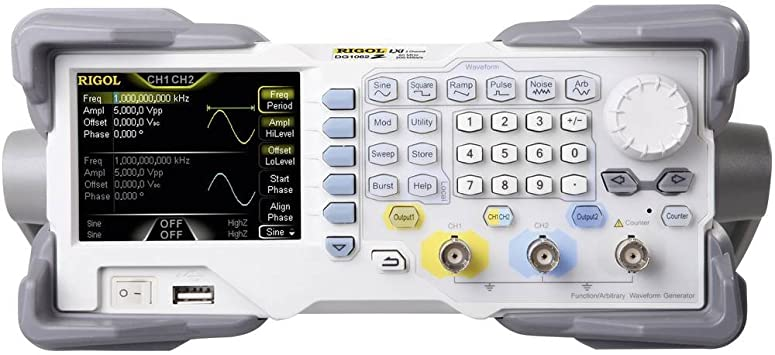
\includegraphics[width=0.5\textwidth]{Figure/GenSeg.jpg}
    \caption{Generatore di segnali DG1032Z Rigol.}
    \label{fig:GenSegnali}
\end{figure}

\subsection{Oscilloscopio}
\begin{figure}[H]
    \centering
    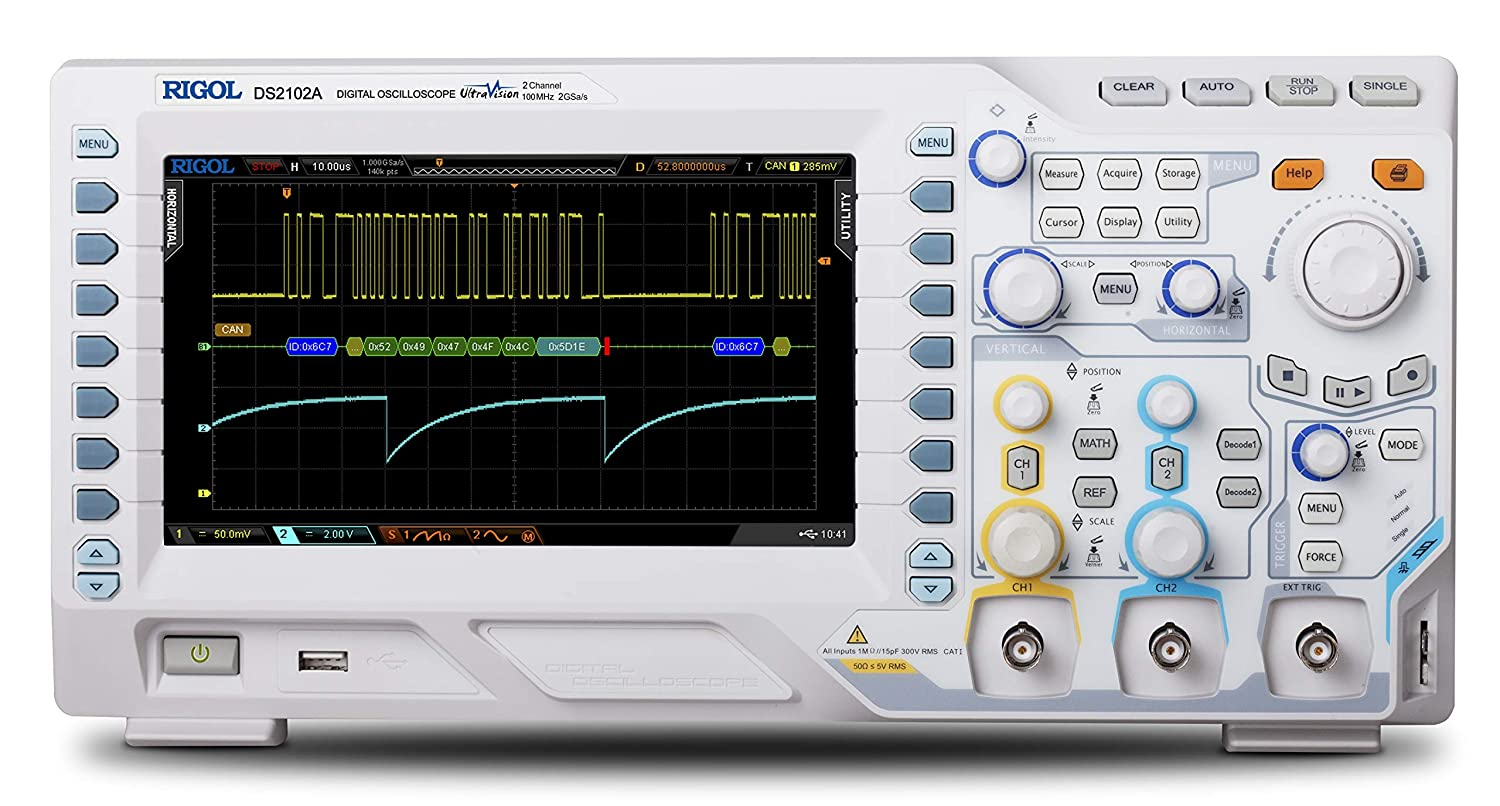
\includegraphics[width=0.5\textwidth]{Figure/Oscilloscopio.jpg}
    \caption{Oscilloscopio DS2102A Rigol.}
    \label{fig:Oscilloscopio}
\end{figure}

\subsection{Componenti elettronici}
\begin{figure}[htbp]
    \centering
    % Prima immagine
    \subfloat[Breadboard\label{fig:breadboard}]{
        \begin{minipage}[c]{0.3\textwidth}
            \centering
            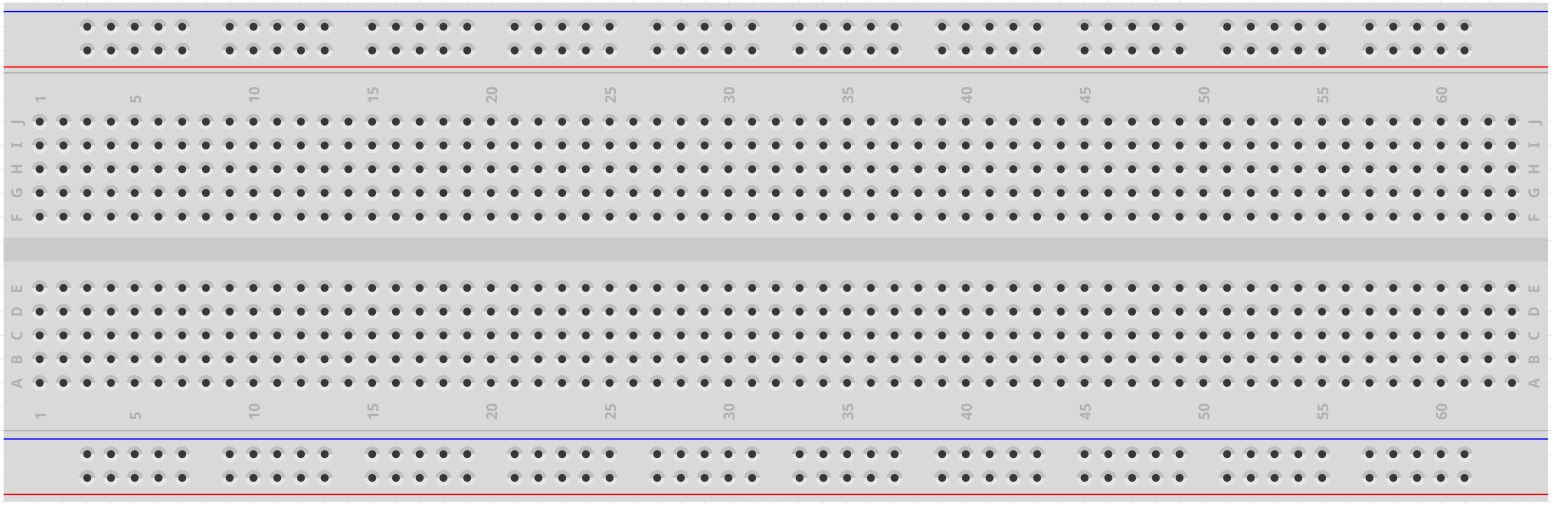
\includegraphics[width=\textwidth]{Figure/breadboard.png}
        \end{minipage}
    }
    \hspace{1.5cm}
    % Seconda immagine
    \subfloat[Diodo\label{fig:diodo}]{
        \begin{minipage}[c]{0.3\textwidth}
            \centering
            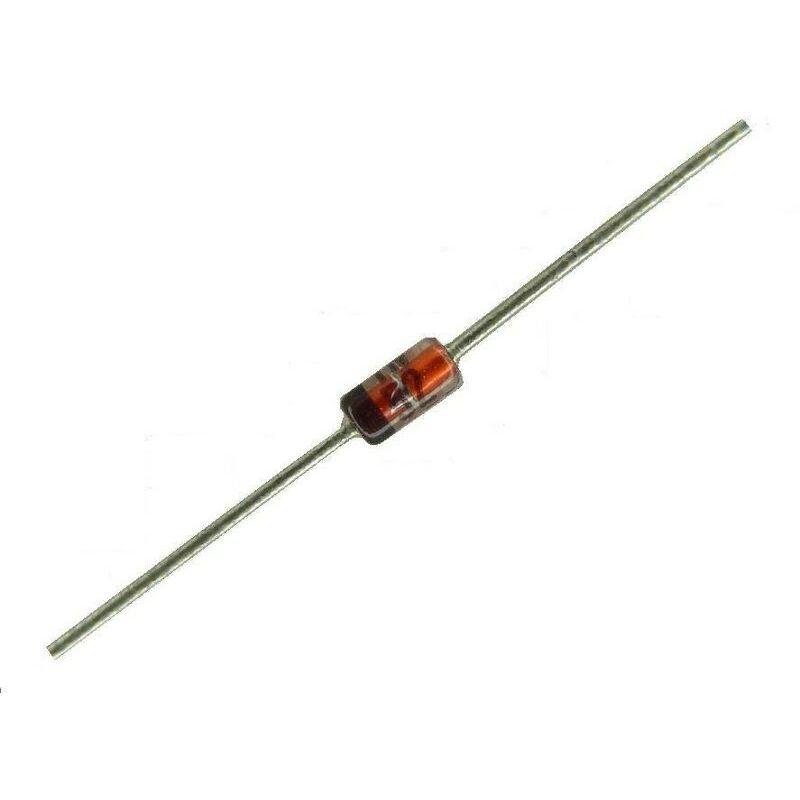
\includegraphics[width=\textwidth]{Figure/diodo.png}
        \end{minipage}
    }
    \caption{Componenti elettronici utilizzati per la costruzione dei circuiti.}
    \label{fig:immagini_affiancate}
\end{figure}

\subsection{Cavetti}
\begin{figure}[htbp]
    \centering
    % Prima immagine
    \subfloat[Cavi coassiali a doppia punta\label{fig:caviRN}]{
        \begin{minipage}[c]{0.3\textwidth}
            \centering
            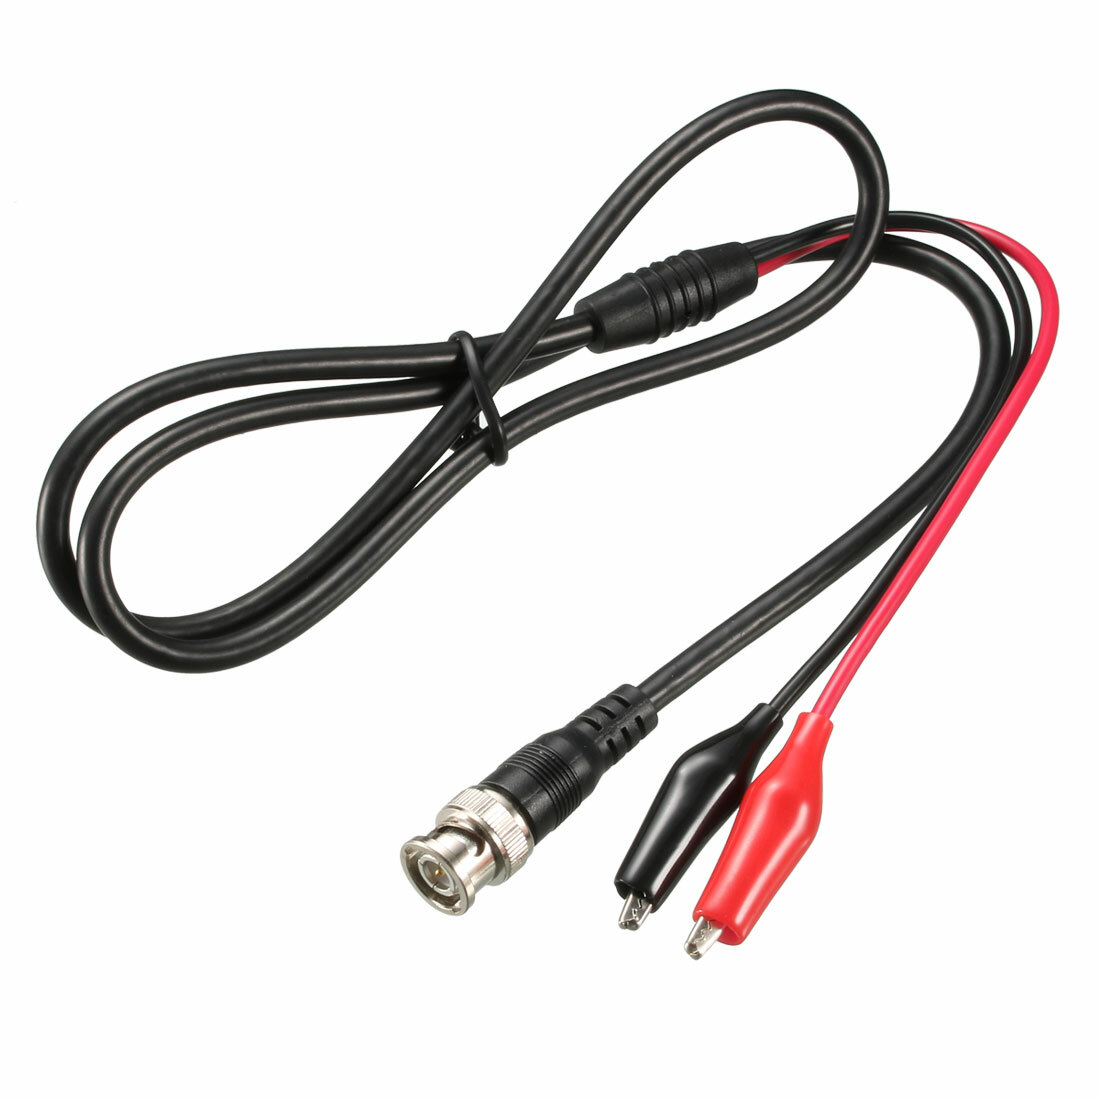
\includegraphics[width=\textwidth]{Figure/caviRossoNero.png}
        \end{minipage}
    }
    \hspace{1.5cm}
    % Seconda immagine
    \subfloat[Cavo coassiale BNC\label{fig:cavo}]{
        \begin{minipage}[c]{0.3\textwidth}
            \centering
            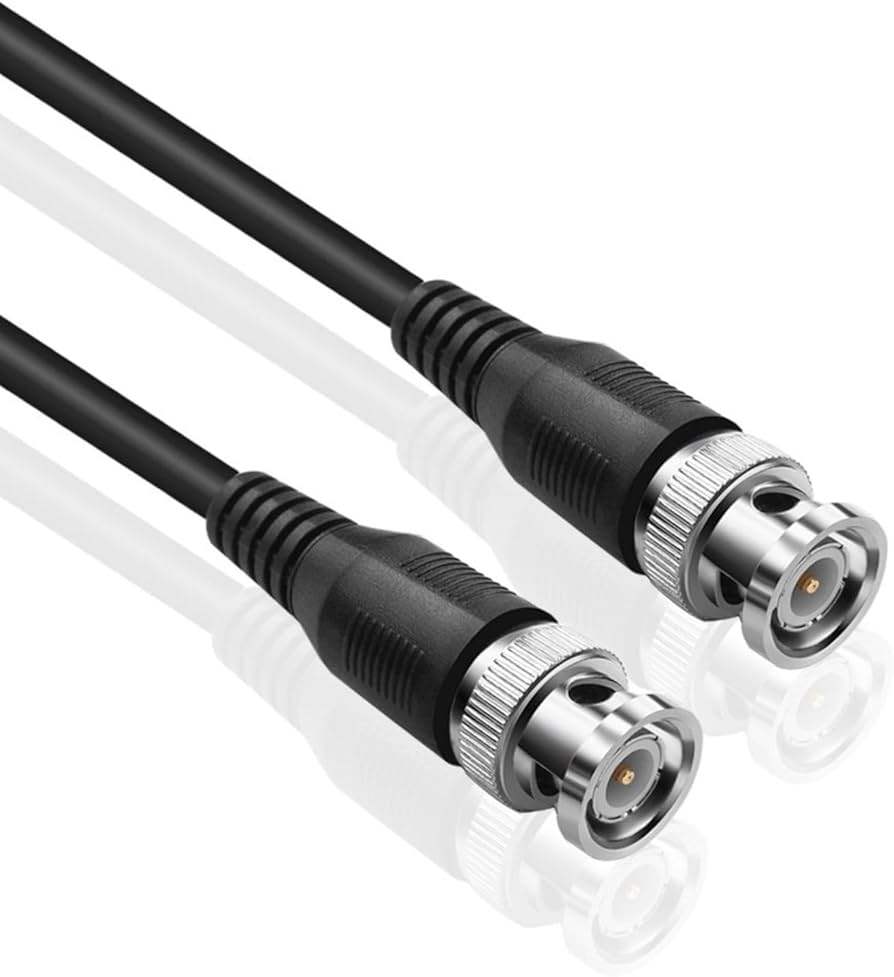
\includegraphics[width=\textwidth]{Figure/cavoBNC.png}
        \end{minipage}
    }
    \caption{Cavetti utilizzati per collegare i componenti elettronici e per le misurazioni.}
    \label{fig:cavi}
\end{figure}

\section{Appendix B\\ Corsi per la sicurezza effettuati}

Gli studenti dichiarano di aver effettuato tutti i corsi della sicurezza che consentono l'utilizzo dei laboratori in cui hanno svolto la propria attività.

\begin{itemize}
    \item Corso Sicurezza base;
    \item Corso sicurezza specifico rischio basso;
    \item corso sicurezza specifico rischio medio.
\end{itemize}

\pagebreak


%-------------------------------------------------------------------------
%	END OF YOUR DOCUMENT
%-------------------------------------------------------------------------
\end{document}